\documentclass[aspectratio=169]{beamer}
\usepackage{capt-of}

% -------------------- Theme / packages --------------------
\usetheme{Madrid}
\usecolortheme{default}
\usefonttheme{professionalfonts}

\usepackage{amsmath, amssymb, bm}
\usepackage{mathtools}
\usepackage{physics} % optional; remove if you prefer
\usepackage{siunitx}
\usepackage{centernot}
\usepackage{tikz}
\usepackage{hyperref}  % robust \href

% -------------------- Handy macros --------------------
\newcommand{\R}{\mathbb{R}}
\newcommand{\x}{\bm{x}}
\newcommand{\X}{\bm{X}}
\newcommand{\I}{\bm{I}}
\newcommand{\uEuler}{\bm{u}}

% Differential operators (Eulerian vs Lagrangian)
\newcommand{\gradx}{\nabla_{\!x}}
\newcommand{\divx}{\nabla_{\!x}\cdot}
\newcommand{\gradX}{\nabla_{\!X}}
\newcommand{\divX}{\nabla_{\!X}\cdot}




% Derivatives

% --- More solid-mechanics tensors (Modules 2--3) ---
\newcommand{\Cten}{\bm{C}}     % right Cauchy-Green
\newcommand{\Bten}{\bm{B}}     % left Cauchy-Green
\newcommand{\Eten}{\bm{E}}     % Green-Lagrange strain
\newcommand{\eten}{\bm{e}}     % Euler-Almansi strain
\newcommand{\sigmaC}{\bm{\sigma}} % Cauchy stress
\newcommand{\Sten}{\bm{S}}     % 2nd Piola-Kirchhoff stress
\newcommand{\Nvec}{\bm{N}}     % reference outward unit normal
\newcommand{\nvec}{\bm{n}}     % current outward unit normal
\newcommand{\tvec}{\bm{t}}     % traction


% --- IMPORTANT NOTATION CHOICE ---
% In IB/IBFE, many authors use F(X,t) for Lagrangian force density.
% To avoid that conflict, we denote the deformation gradient by F_chi.
\newcommand{\Fdef}{\bm{F}_{\chi}}  % deformation gradient = grad_X chi
\newcommand{\Pten}{\bm{P}}         % 1st Piola stress (later)

% IB force densities (used in later modules, reserved here for consistency)
\newcommand{\fEuler}{\bm{f}}       % Eulerian force density on fluid grid
\newcommand{\FLag}{\bm{F}}         % Lagrangian force density on solid mesh

\title[Solid Mechanics for IBFE]{Solid Mechanics You Need for IBFE}
\author{Laura Miller}
\institute{University of Arizona}
\date{\today}

\begin{document}

% ============================================================
% Title
% ============================================================
\begin{frame}
  \titlepage
\end{frame}

\begin{frame}{Resources}
  \begin{itemize}
    \item \href{https://web.iitd.ac.in/~ajeetk/APL104.html}{Solid Mechanics Foundations: UG Solid Mechanics (APL104) – Ajeet Kumar (IIT Delhi).}
    \item \href{https://onlinecourses.nptel.ac.in/noc19_ch27/preview}{NPTEL: Continuum Mechanics and Transport Phenomena (IIT Madras).}
    \item \href{https://www.classcentral.com/course/youtube-modeling-hyperelastic-material-344875}{NPTEL: Computational Continuum Mechanics}
  \end{itemize}
\end{frame}

\begin{frame}{Overview}
\tableofcontents
\end{frame}
% ============================================================
% MODULE 0
% ============================================================
\section{Module 0: What we are doing + notation}

\begin{frame}{Module 0: What this tutorial is (and is not)}
\small
\textbf{Goal:} Build the minimum solid-mechanics toolkit needed to follow IBFE derivations.

\medskip
\textbf{Audience:} advanced undergrads + grad students who are new to continuum mechanics.

\medskip
\textbf{Scope for Modules 0--1:}
\begin{itemize}
\item Set notation and tensor bookkeeping (what is a scalar/vector/tensor; indices).
\item Define reference vs current configuration and the deformation map.
\item Define the deformation gradient \(\Fdef\) and \(J=\det \Fdef\), and what they \emph{mean}.
\item Show how FE approximates \(\chi\) and \(\Fdef\) in IBFE.
\end{itemize}

\end{frame}

\begin{frame}{Notation: configurations, coordinates, and fields}
\small
\begin{columns}[T,onlytextwidth]
  \begin{column}{0.58\textwidth}
    We will use two coordinate systems (two ``worlds''):

    \begin{itemize}
    \item \textbf{Reference/material:} \(B_0\subset\R^d\), \(\X=(X_1,\dots,X_d)\).
    \item \textbf{Current/spatial:} \(B_t\subset\R^d\), \(\x=(x_1,\dots,x_d)\).
    \item \textbf{Motion:} \(\chi(\X,t):B_0\to B_t\), \(\x=\chi(\X,t)\).
    \end{itemize}

    \medskip
    \textbf{Bookkeeping:} \(\X\)-fields live on \(B_0\); \(\x\)-fields live on \(B_t\).
  \end{column}

  \begin{column}{0.42\textwidth}
    \centering
    \vspace{-0.5em} % tweak if needed
    
\includegraphics[width=\linewidth]{pictures/4-2/ref-current.png}\\
    \scriptsize Reference point \(\X\in B_0\) maps to \(\x=\chi(\X,t)\in B_t\).
  \end{column}
\end{columns}
\end{frame}


\begin{frame}{Tensor types and component notation (so you can survive IBFE papers)}
\small

\textbf{Scalars:} \(a \in \R\).

\medskip
\textbf{Vectors:} \(\bm{v}\in \R^d\), components \(v_i\) (spatial) or \(v_I\) (material).

\medskip
\textbf{2nd-order tensors (matrices):}
\begin{itemize}
\item \textbf{Spatial (Eulerian) tensor:} \(\bm{A}\), components \(A_{ij}\) (both indices spatial).
\item \textbf{Material (Lagrangian) tensor:} \(\bm{A}\), components \(A_{IJ}\) (both indices material).
\item \textbf{Mixed / two-point tensor:} components \(A_{iI}\) (maps material directions to spatial directions).
\end{itemize}

\medskip
\textbf{Index convention:}
\begin{itemize}
\item Spatial indices: \(i,j,k \in \{1,\dots,d\}\) (attached to \(\x\)-coordinates).
\item Material indices: \(I,J,K \in \{1,\dots,d\}\) (attached to \(\X\)-coordinates).
\item Summation convention: repeated indices are summed unless stated otherwise.
\end{itemize}
\end{frame}

\begin{frame}{Tensor types and component notation (so you can survive IBFE papers)}
\small
\medskip
\begin{center}
\renewcommand{\arraystretch}{1.15}
\setlength{\tabcolsep}{6pt}
\begin{tabular}{p{0.44\textwidth} p{0.50\textwidth}}
\hline
\textbf{Lives on \(B_0\) (material)} & \textbf{Lives on \(B_t\) (spatial)} \\
\hline
\(\X\) (material coordinate) & \(\x\) (spatial coordinate) \\
\(\chi(\X,t)\) (motion, mapping \(B_0\to B_t\)) & \(\uEuler(\x,t)\) (fluid velocity) \\
\(\Fdef(\X,t)=\gradX\chi(\X,t)\) (mixed tensor, \(F_{iI}\)) & \(\sigmaC(\x,t)\) (Cauchy stress, \(\sigma_{ij}\)) \\
\(J(\X,t)=\det \Fdef\) & \(p(\x,t)\) (pressure) \\
\(\Pten(\X,t)\) (PK1 stress, mixed \(P_{iI}\)) & \(\fEuler(\x,t)\) (Eulerian force density) \\
\hline
\end{tabular}
\end{center}

\end{frame}


\begin{frame}{Material vs spatial derivatives (very common confusion)}
\small
\textbf{Material gradient:} \(\gradX(\cdot)\) means derivatives w.r.t. \(\X\) (reference coordinates).

\medskip
\textbf{Spatial gradient:} \(\gradx(\cdot)\) means derivatives w.r.t. \(\x\) (current coordinates).

\medskip
\textbf{Component forms:}
\[
(\gradX \chi)_{iI} = \pdv{\chi_i}{X_I}, \qquad (\gradx u)_{ij} = \pdv{u_i}{x_j}.
\]

\medskip
\textbf{IBFE heads-up:} Structural kinematics and stresses are typically defined on \(B_0\), so you will often see \(\gradX(\cdot)\) and \(\gradX \cdot (\cdot)\).

\end{frame}


\begin{frame}{Notation note: \(\Fdef\) vs \(\FLag\) in IB/IBFE}
\small
Many immersed boundary (IB) and IBFE papers use \(\FLag(\X,t)\) to denote the \textbf{Lagrangian force density}
defined on the structure mesh. For example, Griffith \& Luo (2017) write the unified weak form as
\[
\int_U \FLag(\X,t)\cdot\bm{V}(\X)\,d\X
= -\int_U \Pten^{\,e}(\X,t)\!:\!\gradX \bm{V}(\X)\,d\X
\]
where \(\Pten^{\,e}=\partial W^e/\partial \bm{F}\) and the symbol \(\bm{F}\) appears \emph{twice} --- once as the deformation gradient and once (as \(\bm{F}(\X,t)\)) as the Lagrangian force density.

\medskip
In solid mechanics, the symbol \(\bm{F}\) is traditionally used for the \textbf{deformation gradient}.
To avoid confusion, in this tutorial we write:
\[
\Fdef(\X,t) := \gradX \chi(\X,t)
\]
for the \textbf{deformation gradient}, and we reserve \(\FLag(\X,t)\) for the \textbf{Lagrangian force density}
(later modules).

\medskip
\textbf{Takeaway:} \(\Fdef\) is kinematics; \(\FLag\) is forcing.
\end{frame}

% ============================================================
% MODULE 1
% ============================================================
\section{Module 1: Configurations and the deformation map}

\begin{frame}{Module 1: Two configurations and a map}
\small
\textbf{Reference configuration:} \(B_0 \subset \R^d\) with material coordinates \(\X\).

\medskip
\textbf{Current configuration:} \(B_t \subset \R^d\) with spatial coordinates \(\x\).

\medskip
\textbf{Motion / deformation map:}
\[
\chi(\X,t): B_0 \to B_t, \qquad \x=\chi(\X,t).
\]

\medskip
\textbf{Displacement:}
\[
\bm{d}(\X,t) = \chi(\X,t) - \X.
\]

\medskip

\end{frame}

% (Preamble reminder if needed)
% \usepackage{graphicx}

\begin{frame}{The deformation gradient $\bm{F}_{\chi}$: differential map and its inverse}
\footnotesize
\begin{columns}[T,onlytextwidth]
  \begin{column}{0.52\textwidth}

  \textbf{Two nearby material points:}
  \[
  \X \in B_0,\qquad \X+d\X \in B_0,
  \qquad d\X := (\X+d\X)-\X.
  \]

  \medskip
  \textbf{Their images under the motion:}
  \[
  \x=\chi(\X,t),\qquad \x+d\chi=\chi(\X+d\X,t),
  \]
  so the \emph{increment} in the current configuration is
  \[
  d\chi := \chi(\X+d\X,t)-\chi(\X,t).
  \]


  \end{column}

  \begin{column}{0.48\textwidth}
  \medskip
  \medskip
  \medskip
  \centering
  % Replace the filename below with wherever you saved the attached image
  
\includegraphics[width=\linewidth]{pictures/4-2/def-tensor.png}

  \vspace{0.25em}
  \scriptsize
  Differential picture: \(\X \mapsto \chi(\X,t)\) and \(\X+d\X \mapsto \chi(\X+d\X,t)\).
  \end{column}
\end{columns}
\end{frame}

\begin{frame}{The deformation gradient $\bm{F}_{\chi}$: differential map and its inverse}
\footnotesize
\begin{columns}[T,onlytextwidth]
  \begin{column}{0.52\textwidth}

  \medskip
  \textbf{Linearization (definition of $\bm{F}_{\chi}$):}
  \[
  \begin{aligned}
  d\chi &\approx \bm{F}_{\chi}(\X,t)\, d\X,\\
  \bm{F}_{\chi}(\X,t) &= \nabla_{\!X}\chi(\X,t).
  \end{aligned}
  \]
  with components
  \[
  (\bm{F}_{\chi})_{iI}(\X,t)=\frac{\partial \chi_i}{\partial X_I}(\X,t).
  \]

  \medskip
  \textbf{Inverse map (when $\chi(\cdot,t)$ is locally invertible):}
  \[
  \begin{aligned}
  d\X &\approx \bm{F}_{\chi}(\X,t)^{-1}\, d\chi,\\
  \bm{F}_{\chi}^{-1}(\x,t) &= \nabla_{\!x}\chi^{-1}(\x,t).
  \end{aligned}
  \]

  \end{column}

  \begin{column}{0.48\textwidth}
  \medskip\medskip\medskip
  \centering
  
\includegraphics[width=\linewidth]{pictures/4-2/def-tensor.png}

  \vspace{0.25em}
  \scriptsize
  Differential picture: \(\X \mapsto \chi(\X,t)\) and \(\X+d\X \mapsto \chi(\X+d\X,t)\).
  \end{column}
\end{columns}
\end{frame}



\begin{frame}{Jacobian \(J=\det\Fdef\): local volume change}
\small
\textbf{Definition:}
\[
J(\X,t)=\det \Fdef(\X,t).
\]

\medskip
\textbf{Meaning:} \(J\) measures local volume ratio (how much a tiny material volume expands/compresses).

\medskip
\textbf{Volume-element transformation:}
\[
dv = J\, dV,
\]
where \(dV\) is a small volume in \(B_0\) and \(dv\) is the corresponding volume in \(B_t\).

\medskip
\textbf{Physical admissibility:} typically require \(J>0\) (no local inversion).

\end{frame}

\begin{frame}{Jacobian determinant $J=\det\Fdef$: area/volume change (stretch)}
\footnotesize
\begin{columns}[T,onlytextwidth]
  \begin{column}{0.45\textwidth}
  \textbf{Idea:} the deformation map sends a small material neighborhood to a small spatial neighborhood.

  \[
  \Fdef(\X,t)=\gradX\chi(\X,t), \qquad
  J(\X,t)=\det\Fdef(\X,t).
  \]

  \textbf{Measure scaling:}
  \[
  da = J\, dA.
  \]
  \scriptsize (In 3D: $dv = J\, dV$.)

  \textbf{Stretch example (2D):} if \(\Fdef=\mathrm{diag}(\lambda_1,\lambda_2)\), then
  \[
  J=\lambda_1\lambda_2.
  \]

  \textbf{Interpretation:}
  \begin{itemize}
    \item \(J>1\): local expansion
    \item \(J<1\): local compression
    \item \(J=1\): locally measure-preserving (volume-preserving in 3D)
  \end{itemize}
  \end{column}

  \begin{column}{0.55\textwidth}
  \centering
\medskip
\medskip
\medskip
\medskip
\medskip
\medskip
  % ---- TikZ picture: explicit bounding box to avoid clipping ----
  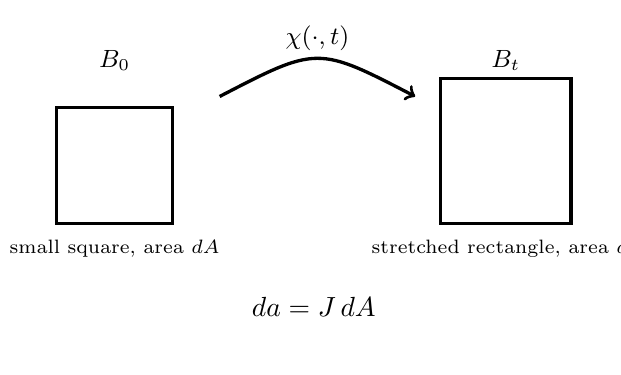
\begin{tikzpicture}[scale=0.92, every node/.style={font=\small}]
    % Make sure Beamer reserves enough space (prevents cut-off)
    \useasboundingbox (-3.6,-1.6) rectangle (4.2,2.8);

    % Left: square in B0
    \node at (-2.4,2.35) {$B_0$};
    \draw[line width=1.1pt] (-3.2,0.1) rectangle (-1.6,1.7);
    \node[font=\scriptsize] at (-2.4,-0.25) {small square, area $dA$};

    % Arrow labeled chi
    \draw[->, line width=1.2pt] (-0.95,1.85) .. controls (0.4,2.55) .. (1.75,1.85);
    \node at (0.4,2.65) {$\chi(\cdot,t)$};

    % Right: rectangle in Bt (pure stretch)
    \node at (3.0,2.35) {$B_t$};
    % Stretch factors: wider and taller than the square
    \draw[line width=1.1pt] (2.1,0.1) rectangle (3.9,2.1);
    \node[font=\scriptsize] at (3.0,-0.25) {stretched rectangle, area $da$};

    % Scaling label
    \node[font=\normalsize] at (0.35,-1.05) {$da = J\, dA$};
  \end{tikzpicture}

  \end{column}
\end{columns}
\end{frame}



\begin{frame}{Micro-check: compute \(\Fdef\) and \(J\) for simple maps}
\small
\textbf{(A) Uniform stretch in 3D:} \(\chi(\X) = (\lambda X_1, \lambda X_2, \lambda X_3)\).
\begin{itemize}
\item What is \(\Fdef\)?
\item What is \(J\)?
\end{itemize}

\medskip
\textbf{(B) Simple shear in 3D:} \(\chi(\X) = (X_1 + \gamma X_2, X_2, X_3)\).
\begin{itemize}
\item Compute \((\Fdef)_{iI}=\partial \chi_i/\partial X_I\).
\item Compute \(J=\det(\Fdef)\).
\end{itemize}


\end{frame}

\begin{frame}{Micro-check: compute \(\Fdef\) and \(J\) for simple maps (solutions)}
\small

\textbf{Recall:} \(\Fdef = \gradX \chi\) with components \((\Fdef)_{iI}=\partial \chi_i/\partial X_I\), and \(J=\det(\Fdef)\).

\medskip
\textbf{(A) Uniform stretch in 3D:} \(\chi(\X) = (\lambda X_1, \lambda X_2, \lambda X_3)\).

\medskip
\emph{Compute \(\Fdef\):}
\[
\Fdef =
\begin{pmatrix}
\frac{\partial \chi_1}{\partial X_1} & \frac{\partial \chi_1}{\partial X_2} & \frac{\partial \chi_1}{\partial X_3}\\
\frac{\partial \chi_2}{\partial X_1} & \frac{\partial \chi_2}{\partial X_2} & \frac{\partial \chi_2}{\partial X_3}\\
\frac{\partial \chi_3}{\partial X_1} & \frac{\partial \chi_3}{\partial X_2} & \frac{\partial \chi_3}{\partial X_3}
\end{pmatrix}
=
\begin{pmatrix}
\lambda & 0 & 0\\
0 & \lambda & 0\\
0 & 0 & \lambda
\end{pmatrix}
= \lambda \I.
\]

\emph{Compute \(J\):}
\[
J=\det(\Fdef)=\det(\lambda \I)=\lambda^3.
\]
\end{frame}

\begin{frame}{Micro-check: compute \(\Fdef\) and \(J\) for simple maps (solutions)}
\medskip
\textbf{(B) Simple shear in 3D:} \(\chi(\X) = (X_1 + \gamma X_2, X_2, X_3)\).

\medskip
\emph{Compute \((\Fdef)_{iI}\):}
\[
\chi_1 = X_1 + \gamma X_2,\quad \chi_2=X_2,\quad \chi_3=X_3.
\]
So
\[
\Fdef=
\begin{pmatrix}
\frac{\partial \chi_1}{\partial X_1} & \frac{\partial \chi_1}{\partial X_2} & \frac{\partial \chi_1}{\partial X_3}\\
\frac{\partial \chi_2}{\partial X_1} & \frac{\partial \chi_2}{\partial X_2} & \frac{\partial \chi_2}{\partial X_3}\\
\frac{\partial \chi_3}{\partial X_1} & \frac{\partial \chi_3}{\partial X_2} & \frac{\partial \chi_3}{\partial X_3}
\end{pmatrix}
=
\begin{pmatrix}
1 & \gamma & 0\\
0 & 1 & 0\\
0 & 0 & 1
\end{pmatrix}.
\]

\emph{Compute \(J\):} this matrix is upper triangular, so its determinant is the product of diagonal entries:
\[
J=\det(\Fdef)=1\cdot 1\cdot 1 = 1.
\]

\medskip
\textbf{Takeaway:} uniform stretch changes volume by \(\lambda^3\), while simple shear preserves volume (\(J=1\)).

\end{frame}


\begin{frame}{Important pitfall: \(\Fdef-\I\) is not ``the strain''}
\small
You will often see (or be tempted to write) \(\Fdef-\I\). Be careful:

\medskip
\textbf{Displacement gradient:}
\[
\gradX \bm{d} = \Fdef - \I.
\]
This is a first derivative of displacement; it is \emph{not} the strain tensor in general.

\medskip
\textbf{Small-deformation (linearized) strain:}
\[
\bm{\varepsilon} = \frac{1}{2}\left(\gradX \bm{d} + (\gradX \bm{d})^{T}\right).
\]

\medskip
\textbf{Takeaway:} For finite deformation, we use nonlinear strain measures (next modules).

\end{frame}



\begin{frame}{Module 1 wrap-up (what you should be fluent with)}
\small
By the end of Module 1, you should be able to:
\begin{itemize}
\item State what \(B_0, B_t, \X, \x, \chi(\X,t)\) mean.
\item Write \(\Fdef=\gradX \chi\) and interpret it as mapping line elements: \(d\x=\Fdef d\X\).
\item Explain \(J=\det\Fdef\) and \(dv = J\,dV\).
\item Keep \(\gradX\) and \(\gradx\) straight.
\item Explain how FE approximates \(\chi\) and \(\Fdef\) in IBFE.
\end{itemize}

\medskip
\textbf{Quick check question:} If \(\chi(\X)=\lambda \X\) in 3D (uniform stretch), what are \(\Fdef\) and \(J\)?
\end{frame}

% ============================================================
% MODULE 2
% ============================================================
\section{Module 2: Strain measures (small vs finite)}

\begin{frame}{Module 2: Why we need nonlinear strain measures}
\small
From Module 1 we have the deformation map \(\chi(\X,t)\) and deformation gradient
\[
\Fdef(\X,t)=\gradX \chi(\X,t).
\]

\medskip
\textbf{Key point:} For \emph{finite} deformations, ``strain'' must:
\begin{itemize}
\item separate stretch from rigid-body rotation (objectivity),
\item behave well under large deformation,
\item reduce to the familiar small-strain tensor when \(\|\gradX \bm{d}\|\ll 1\).
\end{itemize}

\end{frame}

\begin{frame}{Micro-check: rotation vs stretch (what strain should ``feel like'')}
\small
  \centering
  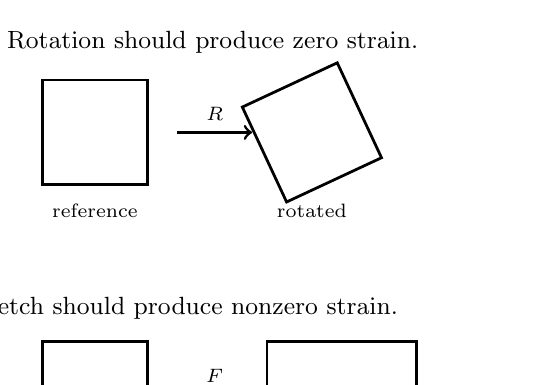
\begin{tikzpicture}[scale=0.95, every node/.style={font=\scriptsize}]
    \useasboundingbox (-3.2,-2.2) rectangle (3.2,2.2);

    % ---------- Panel (i): rotation ----------
    \node[font=\small] at (-2.1,2.0) {(i) Pure rotation: Rotation should produce zero strain.};

    % reference square
    \draw[line width=1.0pt] (-3.0,0.1) rectangle (-1.6,1.5);
    \node at (-2.3,-0.25) {reference};

    % arrow to rotated
    \draw[->, line width=1.0pt] (-1.2,0.8) -- (-0.2,0.8);
    \node at (-0.7,1.05) {$R$};

    % rotated square (same size, rotated)
    \begin{scope}[shift={(0.6,0.8)}, rotate=25]
      \draw[line width=1.0pt] (-0.7,-0.7) rectangle (0.7,0.7);
    \end{scope}
    \node at (0.6,-0.25) {rotated};


    % ---------- Panel (ii): stretch ----------
    \node[font=\small] at (-2.1,-1.55) {(ii) Stretch: Stretch should produce nonzero strain.};

    % reference square (bottom left)
    \draw[line width=1.0pt] (-3.0,-3.4) rectangle (-1.6,-2.0);
    \node at (-2.3,-3.75) {reference};

    % arrow to stretched
    \draw[->, line width=1.0pt] (-1.2,-2.7) -- (-0.2,-2.7);
    \node at (-0.7,-2.45) {$F$};

    % stretched rectangle (bottom right)
    \draw[line width=1.0pt] (0.0,-3.4) rectangle (2.0,-2.0);
    \node at (1.0,-3.75) {stretched};
  \end{tikzpicture}


\end{frame}


\begin{frame}{Reminder: displacement gradient and small (linearized) strain}
\small
Displacement \(\bm{d}(\X,t)=\chi(\X,t)-\X\).

\medskip
Displacement gradient:
\[
\gradX \bm{d} = \Fdef - \I.
\]

\medskip
Small (linearized) strain:
\[
\bm{\varepsilon}=\frac12\left(\gradX \bm{d}+(\gradX \bm{d})^T\right).
\]

\medskip
\textbf{When is this valid?} Roughly when \(\|\gradX \bm{d}\|\ll 1\) (small displacement gradients).


\end{frame}

\begin{frame}{Right and left Cauchy--Green tensors (\(\Cten\) and \(\Bten\))}
\small
Two fundamental stretch tensors built from \(\Fdef\):

\medskip
\textbf{Right Cauchy--Green (reference-friendly):}
\[
\Cten = \Fdef^{T}\Fdef.
\]

\medskip
\textbf{Left Cauchy--Green (current-friendly):}
\[
\Bten = \Fdef \Fdef^{T}.
\]

\medskip
\textbf{Interpretation:} both encode stretch; rigid-body rotations cancel out.

\medskip
\textbf{Frame reminder:} \(\Cten\) naturally pairs with \(\X\)-based descriptions; \(\Bten\) with \(\x\)-based ones.

\end{frame}

\begin{frame}{Green--Lagrange strain \(\Eten\) (reference-frame finite strain)}
\small
\textbf{Definition:}
\[
\Eten = \frac12(\Cten-\I)=\frac12(\Fdef^{T}\Fdef-\I).
\]

\medskip
\textbf{Component form:}
\[
E_{IJ}=\frac12\left(C_{IJ}-\delta_{IJ}\right), \qquad
C_{IJ}=\sum_{i=1}^{d} (\Fdef)_{iI}(\Fdef)_{iJ}.
\]
\medskip
Here \(\delta_{IJ}\) is the Kronecker delta, i.e. \((\I)_{IJ}=\delta_{IJ}\).


\medskip
\textbf{Why it’s useful for IBFE:} \(\Eten\) is defined on the reference configuration and is standard in large-deformation elasticity.

\end{frame}

\begin{frame}{Green--Lagrange strain $\Eten$: geometric meaning}
\small
\begin{columns}[T,onlytextwidth]
  \begin{column}{0.56\textwidth}
  \textbf{Definition:}
  \[
  \Eten=\tfrac12(\Cten-\I),\qquad \Cten = \Fdef^{T}\Fdef,\qquad \Fdef=\gradX\chi.
  \]

  \medskip
  \textbf{Key interpretation: change in squared length.}

  For a material line element \(d\X\),
  \[
  d\x = \Fdef\, d\X,
  \qquad
  |d\x|^2 - |d\X|^2
  \;=\;
  2\, d\X^T \Eten\, d\X.
  \]

  \medskip
  \textbf{So:} \(\Eten=0\) means all small material lengths are preserved (rigid motion: rotation + translation).
  \end{column}

  \begin{column}{0.44\textwidth}
  \centering
  
\includegraphics[width=\linewidth]{pictures/4-2/Green-Lagrange.png}\\
  \end{column}
\end{columns}
\end{frame}



\begin{frame}{Euler--Almansi strain \(\eten\) (current-frame finite strain)}
\small
A commonly used \emph{spatial} (current-frame) finite strain is the Euler--Almansi strain:
\[
\eten = \frac12\left(\I-\Bten^{-1}\right)
      = \frac12\left(\I-(\Fdef\Fdef^T)^{-1}\right).
\]

\medskip
\textbf{Rule of thumb for IBFE derivations:} it is often more convenient to work in the reference frame with \(\Fdef\), \(\Cten\), and \(\Eten\).

\end{frame}

\begin{frame}{Euler--Almansi strain $\bm{e}$: geometric meaning (spatial strain)}
\small

\textbf{Definition (lives on $B_t$):}
\[
\bm{e} = \tfrac12\bigl(\bm{I} - \bm{B}^{-1}\bigr),
\qquad
\bm{B} = \bm{F_\chi}\,\bm{F_\chi}^{T}.
\]

\medskip
\textbf{Key interpretation: change in squared length, expressed in the current configuration.}

Take a small \emph{spatial} line element \(d\bm{x}\) in \(B_t\). The corresponding material line element is
\[
d\bm{X} = \bm{F_\chi}^{-1}\, d\bm{x}.
\]
Compare squared lengths:
\[
|d\bm{x}|^2 - |d\bm{X}|^2
= d\bm{x}\cdot(\bm{I}-\bm{B}^{-1})\,d\bm{x}
= 2\, d\bm{x}\cdot \bm{e}\, d\bm{x}.
\]

\medskip
\textbf{Sanity check:} if \(\bm{F}= \bm{R}\) is a pure rotation, then \(\bm{B}=\bm{R}\bm{R}^T=\bm{I}\) and \(\bm{e}=\bm{0}\).

\medskip
\textbf{Bridge to Green--Lagrange strain:}
\[
\bm{e} = \bm{F_\chi}^{-T}\,\bm{E}\,\bm{F_\chi}^{-1}.
\]
\end{frame}



\begin{frame}{Micro-check 1: pure rotation should give zero strain}
\small
Let \(\chi(\X)=\bm{R}\X\), where \(\bm{R}\) is a rotation matrix (\(\bm{R}^T\bm{R}=\I\), \(\det\bm{R}=1\)).

\medskip
Compute:
\[
\Fdef=\gradX\chi=\bm{R},\qquad
\Cten=\Fdef^T\Fdef=\bm{R}^T\bm{R}=\I,\qquad
\Eten=\frac12(\Cten-\I)=\bm{0}.
\]

\medskip
\textbf{Takeaway:} \(\Eten\) is objective (it ignores rigid-body rotations).

\end{frame}




\begin{frame}{Micro-check 2: simple shear}
\small
Consider simple shear in 2D (extend to 3D by adding \(x_3=X_3\)):
\[
\chi(\X) = \begin{pmatrix} X_1+\gamma X_2 \\ X_2 \end{pmatrix}.
\]

Then
\[
\Fdef=
\begin{pmatrix}
1 & \gamma \\
0 & 1
\end{pmatrix},
\qquad
\Cten=\Fdef^T\Fdef=
\begin{pmatrix}
1 & \gamma \\
\gamma & 1+\gamma^2
\end{pmatrix}.
\]

So
\[
\Eten=\frac12(\Cten-\I)=\frac12
\begin{pmatrix}
0 & \gamma \\
\gamma & \gamma^2
\end{pmatrix}.
\]

\medskip
\textbf{Observation:} off-diagonal terms scale like \(\gamma\), but \emph{finite strain} also includes the \(\gamma^2\) term.

\end{frame}

\begin{frame}{Strain invariants (for isotropic hyperelasticity)}
\small
For isotropic hyperelastic models, energies are often written in terms of invariants of \(\Cten\) (or \(\Bten\)).

\medskip
Standard invariants of \(\Cten\):
\[
I_1 = \mathrm{tr}(\Cten), \qquad
I_2 = \frac12\left[(\mathrm{tr}\,\Cten)^2 - \mathrm{tr}(\Cten^2)\right], \qquad
I_3 = \det(\Cten)=J^2,
\]
where \(J=\det(\Fdef)\).

\medskip
\textbf{Interpretation:}
\begin{itemize}
\item \(I_3\) encodes volume change (\(J\)).
\item \(I_1, I_2\) encode distortional (shape) changes.
\end{itemize}


\end{frame}

\begin{frame}{Module 2 wrap-up}
\small
You should now be able to:
\begin{itemize}
\item distinguish \(\gradX\bm{d}=\Fdef-\I\) from strain,
\item define \(\Cten=\Fdef^T\Fdef\) and \(\Bten=\Fdef\Fdef^T\),
\item compute \(\Eten=\tfrac12(\Cten-\I)\) for finite strain in the reference frame,
\item recognize the spatial strain \(\eten=\tfrac12(\I-\Bten^{-1})\),
\item use invariants \(I_1,I_2,I_3\) (and remember \(I_3=J^2\)).
\end{itemize}

\medskip
\textbf{Quick check:} If \(J=1\), what is \(I_3\)?
\end{frame}

% ============================================================
% MODULE 3
% ============================================================
\section{Module 3: Stress measures and transformations}

\begin{frame}{Module 3: Why so many stresses?}
\small
In fluid mechanics you typically use the Cauchy stress \(\sigmaC(\x,t)\) (defined on the current configuration).

\medskip
In IBFE, the structural mechanics is often computed in the \emph{reference} frame using:
\begin{itemize}
\item first Piola--Kirchhoff stress \(\Pten(\X,t)\) (reference-frame traction mapping),
\item sometimes second Piola--Kirchhoff stress \(\Sten(\X,t)\) (pairs naturally with \(\Eten\)).
\end{itemize}

\medskip
\textbf{Goal of this module:} connect \(\sigmaC\), \(\Pten\), and \(\Sten\) cleanly, and keep track of frames.

\end{frame}

\begin{frame}{Cauchy stress \(\sigmaC\) and traction}
\small
\textbf{Cauchy stress:} \(\sigmaC(\x,t)\) is defined in the current configuration \(B_t\).

\medskip
\textbf{Traction on a surface:} if \(\nvec\) is the outward unit normal (current configuration),
\[
\tvec(\x,t;\nvec) = \sigmaC(\x,t)\,\nvec.
\]

\medskip
\textbf{Differential force on an area element \(da\):}
\[
d\bm{f} = \sigmaC \nvec \, da.
\]
\end{frame}

\begin{frame}{Traction vectors and Cauchy's stress law}
\centering


\includegraphics[width=0.6\textwidth]{pictures/4-2/traction-vectors.png}

\vspace{0.5em}
\scriptsize
Source: \href{https://pkel015.connect.amazon.auckland.ac.nz/SolidMechanicsBooks/Part_III/Chapter_3_Stress_Mass_Momentum/Stress_Balance_Principles_03_The_Cauchy_Stress_Tensor.pdf}{Solid Mechanics Books, Part III: Chapter 3 (Auckland)}.
\end{frame}


\begin{frame}{First Piola--Kirchhoff stress \(\Pten\) (PK1)}
\small
\textbf{First Piola--Kirchhoff stress:} \(\Pten(\X,t)\) is defined on the reference configuration \(B_0\).

\medskip
It maps \emph{reference} normals/areas to force. If \(\Nvec\) is the outward unit normal in the reference configuration and \(dA\) is reference area,
\[
d\bm{f} = \Pten(\X,t)\,\Nvec\, dA.
\]

\medskip
\textbf{Important note:} \(\Pten\) is generally \emph{not symmetric}.

\end{frame}

\begin{frame}{Traction on matching surface patches: Cauchy vs. Piola stress}
\small
\begin{columns}[T,onlytextwidth]
  \begin{column}{0.50\textwidth}
  \textbf{Same physical force on a corresponding surface patch}

  \medskip
  \textbf{Current (spatial) configuration $B_t$:}
  \[
  d\bm{f} = \bm{t}\,da,
  \qquad
  \bm{t}(\bm{n}) = \sigmaC\,\bm{n}.
  \]
  (\(\bm{t}\) is traction per \emph{current} area \(da\).)

  \medskip
  \textbf{Reference (material) configuration $B_0$:}
  \[
  d\bm{f} = \bm{T}\,dA,
  \qquad
  \bm{T}(\bm{N}) = \Pten\,\bm{N}.
  \]
  (\(\bm{T}\) is traction per \emph{reference} area \(dA\).)

  \medskip
  \textbf{Full bridge (stress measure conversion):}
  \[
  \Pten = J\,\sigmaC\,\Fdef^{-T},
  \qquad
  J=\det\Fdef.
  \]

  \end{column}

  \begin{column}{0.50\textwidth}
  \medskip
\medskip
\medskip
\medskip
\medskip
\medskip
\medskip
\medskip
  \centering
  
\includegraphics[width=\linewidth]{pictures/4-2/traction-vectors-B0-B1.png}

  \vspace{0.4em}
  \scriptsize
  Source: \href{https://pkel015.connect.amazon.auckland.ac.nz/SolidMechanicsBooks/Part_III/Chapter_3_Stress_Mass_Momentum/Stress_Balance_Principles_03_The_Cauchy_Stress_Tensor.pdf}{Solid Mechanics Books, Part III: Chapter 3 (Auckland)}.
  \end{column}
\end{columns}
\end{frame}


\begin{frame}{Nanson's formula: how oriented area transforms}
\small

\textbf{Why we need it:} To equate the \emph{same physical force} written on corresponding patches:
\[
d\bm{f} = \sigmaC\,\nvec\,da
\qquad \text{and} \qquad
d\bm{f} = \Pten\,\Nvec\,dA.
\]
So we need a relation between the \emph{oriented area vectors} \(\nvec\,da\) and \(\Nvec\,dA\).

\medskip
\textbf{Nanson's formula (area transformation):}
\[
\nvec\, da = J\, \Fdef^{-T}\, \Nvec\, dA,
\qquad J=\det(\Fdef).
\]

\medskip
\textbf{Geometric interpretation:}
\begin{itemize}
\item The vector \(\Nvec\,dA\) is the \emph{oriented area} of a tiny patch in \(B_0\).
\item Under the map \(d\x=\Fdef\,d\X\), the patch edges transform by \(\Fdef\).
\item The mapped cross product gives the new oriented area:
      \(\;(\Fdef\,d\X_1)\times(\Fdef\,d\X_2)=J\,\Fdef^{-T}(d\X_1\times d\X_2)\).
\end{itemize}

\medskip
\textbf{Takeaway:} Nanson is exactly the tool that converts \(\sigmaC\,\nvec\,da\) into a reference-area form.
\end{frame}


\begin{frame}{Piola transform: relation between \(\sigmaC\) and \(\Pten\)}
\small
Start from equality of the same physical force:
\[
d\bm{f}=\sigmaC\nvec\, da = \Pten\Nvec\, dA.
\]
Using Nanson's formula \(\nvec da = J\Fdef^{-T}\Nvec dA\), we obtain:
\[
\Pten = J\,\sigmaC\,\Fdef^{-T}.
\]

Equivalently,
\[
\sigmaC = \frac{1}{J}\,\Pten\,\Fdef^{T}.
\]
\end{frame}

\begin{frame}{Second Piola--Kirchhoff stress \(\Sten\) (useful with \(\Eten\))}
\small
Define the second Piola--Kirchhoff stress:
\[
\Sten = \Fdef^{-1}\Pten.
\]

Equivalently,
\[
\Pten = \Fdef\,\Sten.
\]

\medskip
\textbf{Why it’s useful:} \(\Sten\) lives in the reference frame and is often symmetric for many hyperelastic materials
(because it pairs naturally with \(\Eten\)).

\end{frame}

\begin{frame}{Micro-check: dimensional and symmetry sanity checks}
\small
\textbf{Check 1 (units):}
\begin{itemize}
\item \(\sigmaC\) is force per \emph{current} area.
\item \(\Pten\) is force per \emph{reference} area (because \(\Pten \Nvec dA\) is a force).
\end{itemize}

\medskip
\textbf{Check 2 (symmetry):}
\begin{itemize}
\item \(\sigmaC\) is symmetric in standard (non-polar) continua --- this follows from balance of angular momentum.
\item \(\Pten\) is generally \emph{not} symmetric even when \(\sigmaC\) is symmetric (because of the \(\Fdef^{-T}\) mapping in \(\Pten = J\sigmaC\Fdef^{-T}\)). The symmetry condition for \(\Pten\) reads \(\Pten\Fdef^T = \Fdef\Pten^T\).
\item \(\Sten = \Fdef^{-1}\Pten\) \emph{is} symmetric whenever \(\sigmaC\) is symmetric (one reason it pairs naturally with \(\Eten\)).
\end{itemize}

\end{frame}

\begin{frame}{Module 3 wrap-up}
\small
You should now be able to:
\begin{itemize}
\item define traction \(\tvec=\sigmaC\nvec\) on \(B_t\),
\item interpret \(\Pten\) via \(d\bm{f}=\Pten\Nvec dA\) on \(B_0\),
\item use Nanson's formula \(\nvec da = J\Fdef^{-T}\Nvec dA\),
\item convert stresses using the Piola transform:
\[
\Pten = J\sigmaC\Fdef^{-T}, \qquad \sigmaC = \frac{1}{J}\Pten\Fdef^T,
\]
\item define the second Piola stress \(\Sten=\Fdef^{-1}\Pten\) (and \(\Pten=\Fdef\Sten\)).
\end{itemize}

\medskip
\textbf{Quick check:} If \(J=1\), how does \(\Pten\) relate to \(\sigmaC\)?
\end{frame}


% -----------------------------------------------------------
% ------------------------------------------------------------
% ============================================================
% Add this slide inside Module 3 (right after "Module 3: Why so many stresses?"
% is a good spot).
% ============================================================

\begin{frame}{IBFE notation bridge}
\small
Different communities reuse the same symbols. Here is the translation map we will use in this tutorial.

\medskip
\textbf{Kinematics (solid mechanics):}
\[
\Fdef(\X,t) := \gradX \chi(\X,t)
\quad\text{(deformation gradient).}
\]

\medskip
\textbf{Forcing (IB/IBFE):}
\begin{itemize}
\item \(\FLag(\X,t)\): \textbf{Lagrangian force density} defined on the structure mesh (many IB/IBFE papers write this as \(\bm{F}(\X,t)\)).
\item \(\fEuler(\x,t)\): \textbf{Eulerian force density} applied in the fluid momentum equation.
\end{itemize}

\medskip
\textbf{Stresses (this module):}
\[
\sigmaC(\x,t)\ \text{(Cauchy, current)};\qquad
\Pten(\X,t)\ \text{(PK1, reference)};\qquad
\Sten(\X,t)\ \text{(PK2, reference)}.
\]

\medskip
\textbf{Takeaway:} In what follows, \(\Fdef\) is always kinematics, while \(\FLag\) and \(\fEuler\) are always forces.
\end{frame}

% ============================================================
% MODULE 4
% ============================================================
\section{Module 4: Hyperelasticity (energy \texorpdfstring{$\to$}{->} stress)}

\begin{frame}{Module 4: What is hyperelasticity?}
\small
\textbf{Hyperelastic material:} stress is derived from a stored-energy (strain-energy) density.

\medskip
We prescribe a scalar energy density per \emph{reference volume}:
\[
W(\Fdef) \quad \left[\frac{\text{energy}}{\text{reference volume}}\right],
\]
and define the first Piola--Kirchhoff stress by
\[
\Pten(\X,t) = \pdv{W}{\Fdef}\big(\Fdef(\X,t)\big).
\]

\medskip
\textbf{Key idea:} the constitutive law is encoded in one scalar function \(W\).


\end{frame}

% -------------------------
% Slide 1: What is dW/dF? Component form + "shape check"
% -------------------------
\begin{frame}{What does $\partial W/\partial \bm{F}_{\chi}$ mean? (components and shapes)}
\footnotesize

\textbf{Setup:} The strain energy density is a scalar-valued function of a matrix:
\[
W:\R^{d\times d}\to \R,\qquad \bm{F}_{\chi}\mapsto W(\bm{F}_{\chi}).
\]

\medskip
\textbf{Component definition:} The derivative \(\dfrac{\partial W}{\partial \bm{F}_{\chi}}\) is a \emph{2nd-order tensor}
(same shape as \(\bm{F}_{\chi}\)) with components
\[
\left(\frac{\partial W}{\partial \bm{F}_{\chi}}\right)_{iI}
\;:=\;
\frac{\partial W}{\partial (\bm{F}_{\chi})_{iI}}.
\]

\medskip
Equivalently, if we view \(W\) as a function of the \(d^2\) scalar variables \((\bm{F}_{\chi})_{iI}\), then
\[
\frac{\partial W}{\partial \bm{F}_{\chi}}
=
\begin{pmatrix}
\frac{\partial W}{\partial (\bm{F}_{\chi})_{11}} & \cdots & \frac{\partial W}{\partial (\bm{F}_{\chi})_{1d}}\\
\vdots & \ddots & \vdots\\
\frac{\partial W}{\partial (\bm{F}_{\chi})_{d1}} & \cdots & \frac{\partial W}{\partial (\bm{F}_{\chi})_{dd}}
\end{pmatrix}.
\]

\medskip
\textbf{Shape check (dimensions):}
\[
W\in\R,\qquad \bm{F}_{\chi}\in\R^{d\times d},\qquad
\frac{\partial W}{\partial \bm{F}_{\chi}}\in\R^{d\times d}.
\]

\medskip
\textbf{In IBFE:} the first Piola--Kirchhoff stress is $\bm{P} := \frac{\partial W}{\partial \bm{F}_{\chi}}.$
\end{frame}


% -------------------------
% Slide 2: Directional derivative + meaning of ":" (Frobenius inner product)
% -------------------------
\begin{frame}{Directional derivative viewpoint and the meaning of ``$: $''}
\footnotesize

\textbf{Directional derivative viewpoint:} perturb \(\bm{F}_{\chi}\) in a direction \(\delta\bm{F}_{\chi}\) and look at the first-order change:
\[
\delta W
\;:=\;
\left.\frac{d}{d\varepsilon}W\!\left(\bm{F}_{\chi}+\varepsilon\,\delta\bm{F}_{\chi}\right)\right|_{\varepsilon=0}.
\]

\medskip
\textbf{Definition of the gradient w.r.t.\ a matrix:} \(\dfrac{\partial W}{\partial \bm{F}_{\chi}}\) is defined to be the unique matrix satisfying
\[
\delta W
=
\frac{\partial W}{\partial \bm{F}_{\chi}} : \delta\bm{F}_{\chi}
\qquad \text{for all } \delta\bm{F}_{\chi}.
\]

\medskip
\textbf{What does ``$: $'' mean here?} It is the \emph{double contraction} (Frobenius inner product) of two matrices:
\[
\bm{A}:\bm{B}
\;:=\;
\sum_{i,I} A_{iI}B_{iI}
\;=\;
\mathrm{tr}(\bm{A}^{T}\bm{B}).
\]

\medskip
\textbf{So in components:}
\[
\delta W
=
\sum_{i,I}\left(\frac{\partial W}{\partial (\bm{F}_{\chi})_{iI}}\right)\delta(\bm{F}_{\chi})_{iI}.
\]

\medskip
\textbf{Takeaway (IBFE notation):} $\bm{P}=\frac{\partial W}{\partial \bm{F}_{\chi}}
\quad\Longleftrightarrow\quad
\delta W = \bm{P}:\delta\bm{F}_{\chi}.$
\end{frame}


\begin{frame}{Objectivity (frame indifference) and isotropy}
\small
A basic physical requirement:

\medskip
\textbf{Objectivity:} superposing a rigid-body rotation should not change stored energy:
\[
W(\bm{R}\Fdef)=W(\Fdef)\quad \text{for all rotations }\bm{R}\in SO(d).
\]

\medskip
A common way to guarantee objectivity is to write \(W\) as a function of \(\Cten=\Fdef^T\Fdef\):
\[
W(\Fdef)=\widehat{W}(\Cten).
\]

\medskip
\textbf{Isotropy:} material has no preferred directions (in reference frame). For isotropic hyperelasticity,
\[
\widehat{W}(\Cten)=\widehat{W}(I_1,I_2,I_3),
\]
where \(I_1,I_2,I_3\) are invariants of \(\Cten\) (Module 2).

\end{frame}

\begin{frame}{Compressible vs (nearly) incompressible response}
\small
Recall \(J=\det(\Fdef)\).

\medskip
\textbf{Compressible:} volume changes are allowed; \(W\) penalizes compression/expansion through terms involving \(J\).

\medskip
\textbf{Incompressible:} enforce
\[
J=1
\]
exactly (constraint), typically via a Lagrange multiplier (pressure-like field) in the solid.

\medskip
\textbf{Nearly incompressible (common in IBFE):} use a \emph{penalty} that strongly discourages \(J\neq 1\):
\[
W(\Fdef) = W_{\mathrm{iso}}(\text{shape change}) + W_{\mathrm{vol}}(J).
\]

\medskip
\textbf{Note (IBFE-specific):} Because the fluid is incompressible (\(\divx\uEuler = 0\)) and the structure moves with the fluid (\(\partial \chi/\partial t = \uEuler\circ\chi\)), the continuous IBFE formulation already implies \(J\equiv 1\). However, the \emph{discrete} scheme typically allows volumetric drift, so the volumetric energy \(W_{\mathrm{vol}}(J)\) is best viewed as a \textbf{stabilization} term and \(\kappa\) as a stabilization parameter rather than a true bulk modulus (Griffith \& Patankar 2020).

\end{frame}

\begin{frame}{Modified deformation gradient \(\bar{\bm{F}}\) (volume--deviatoric split)}
\small
A useful trick for nearly incompressible IBFE: multiplicatively split \(\Fdef\) into volumetric and isochoric (volume-preserving) parts,
\[
\Fdef = J^{1/3}\,\bar{\Fdef},\qquad
\bar{\Fdef} := J^{-1/3}\,\Fdef,
\qquad \det \bar{\Fdef} = 1.
\]

\medskip
\textbf{Why this matters in IBFE:} Build the shearing energy from \emph{modified} invariants
\[
\bar{I}_1 = \mathrm{tr}(\bar{\Cten}),\quad \bar{I}_2 = \tfrac12\bigl((\mathrm{tr}\,\bar{\Cten})^2-\mathrm{tr}(\bar{\Cten}^2)\bigr),\qquad \bar{\Cten} = \bar{\Fdef}^T \bar{\Fdef},
\]
so that the shearing part \(W(\bar{\Fdef})\) is by construction insensitive to volume change, and the volumetric stabilization \(W_{\mathrm{vol}}(J)\) is the \emph{only} term that responds to \(J\neq 1\).

\medskip
\textbf{Result reported by Griffith \& Patankar (2020):} For nearly incompressible IBFE, using both modified invariants \emph{and} a volumetric stabilization yields accuracy comparable to standard stabilized FEM for incompressible elasticity (e.g., the twisted beam / Mooney--Rivlin benchmark of Bonet et al.\ 2015).

\end{frame}

\begin{frame}{Volumetric penalty $W_{\mathrm{vol}}(J)$: enforcing near-incompressibility}
\small

\begin{columns}[T,onlytextwidth]
  \begin{column}{0.50\textwidth}
  \textbf{Idea:} add a volumetric energy that strongly penalizes volume change.
  \[
  J=\det(\bm{F}),\qquad
  W_{\mathrm{vol}}(J)\ \text{has a sharp minimum at } J=1.
  \]

  \medskip
  \textbf{Interpretation:}
  \begin{itemize}
    \item \(J=1\): locally volume-preserving (incompressible limit)
    \item \(J>1\): local expansion \(\Rightarrow\) penalty increases
    \item \(J<1\): local compression \(\Rightarrow\) penalty increases
  \end{itemize}

  \medskip
  \textbf{Two common choices:}
  \[
  W_{\mathrm{vol}}(J)=\frac{\kappa}{2}(J-1)^2
  \quad\text{or}\quad
  W_{\mathrm{vol}}(J)=\frac{\kappa}{2}(\ln J)^2.
  \]
  \scriptsize Both satisfy \(W_{\mathrm{vol}}(1)=W'_{\mathrm{vol}}(1)=0\), so no extra energy/stress is added at \(J=1\). We use the \(\ln J\) form for the neo-Hookean below; it is the choice used in the IBFE literature (Griffith \& Patankar 2020).
  \end{column}

  \begin{column}{0.50\textwidth}
  \centering
  
\includegraphics[width=\linewidth]{pictures/4-2/Wvol_J_plot.png}
  \end{column}
\end{columns}
\end{frame}


\begin{frame}{A standard example: compressible neo-Hookean energy}
\small
One widely used compressible neo-Hookean model (per reference volume):
\[
W(\Fdef)=\frac{\mu}{2}(I_1-3)-\mu\ln J+\frac{\kappa}{2}(\ln J)^2,
\]
where
\[
I_1=\mathrm{tr}(\Cten),\quad \Cten=\Fdef^T\Fdef,\quad J=\det(\Fdef).
\]

\medskip
Parameters:
\begin{itemize}
\item \(\mu>0\): shear modulus (controls distortional stiffness),
\item \(\kappa>0\): bulk modulus (controls volumetric stiffness).
\end{itemize}

\end{frame}

\begin{frame}{Neo-Hookean stress: a useful closed form for \(\Pten\)}
\small
For the neo-Hookean energy
\[
W(\Fdef)=\frac{\mu}{2}(I_1-3)-\mu\ln J+\frac{\kappa}{2}(\ln J)^2,
\]
a standard expression for the first Piola stress is:
\[
\Pten = \mu\left(\Fdef-\Fdef^{-T}\right)+\kappa(\ln J)\,\Fdef^{-T}.
\]

\medskip
\textbf{Shape check:} \(\Pten\in\R^{d\times d}\), same as \(\Fdef\).

\medskip
\textbf{Special case:} if \(J=1\), this reduces to \(\Pten=\mu(\Fdef-\Fdef^{-T})\).

\end{frame}

\begin{frame}{From \(\Pten\) to other stresses (connect to Module 3)}
\small
Once \(\Pten\) is known, we can map between stress measures.

\medskip
Second Piola:
\[
\Sten = \Fdef^{-1}\Pten.
\]

\medskip
Cauchy stress:
\[
\sigmaC = \frac{1}{J}\,\Pten\,\Fdef^T
       = \frac{1}{J}\,\pdv{W}{\Fdef}\,\Fdef^T.
\]
\scriptsize (The right-hand expression goes directly from energy to Cauchy stress, bypassing \(\Pten\); see Griffith \& Patankar 2020.)

\medskip
\small
\textbf{Interpretation:} \(\Pten\) is convenient to compute in the reference frame; \(\sigmaC\) is what appears naturally in current-frame balance laws.

\end{frame}



% ============================================================
% Add this as the LAST slide of Module 4 (right before Module 4 wrap-up,
% or replace the "Next:" line in the wrap-up slide).
% ============================================================

\begin{frame}{IBFE pipeline preview: energy \texorpdfstring{$\to$}{->} stress \texorpdfstring{$\to$}{->} nodal forces \texorpdfstring{$\to$}{->} fluid forcing}
\footnotesize
Here is the end-to-end IBFE ``force pipeline'' you should keep in mind:

\medskip
\textbf{(1) Kinematics from the FE deformation map}
\[
\chi_h(\X,t)\ \Rightarrow\ \Fdef{}_h(\X,t)=\gradX\chi_h(\X,t)\ \Rightarrow\ J_h=\det(\Fdef{}_h).
\]

\medskip
\textbf{(2) Constitutive law via a hyperelastic energy}
\[
W(\Fdef{}_h)\ \Rightarrow\ \Pten_h(\X,t)=\pdv{W}{\Fdef}\Big|_{\Fdef=\Fdef{}_h(\X,t)}.
\]

\medskip
\textbf{(3) Convert stress to \emph{nodal forces} using the weak form (finite elements)}
\[
\text{weak form:}\quad \int_{B_0} \Pten_h : \gradX \bm{\phi}_m\, dV
\ \Rightarrow\ \text{nodal force vector(s)}.
\]

\medskip
\textbf{(4) IB coupling: spread to the fluid and interpolate velocities back}
\[
\text{nodal forces} \Rightarrow \FLag(\X,t)\Rightarrow \fEuler(\x,t)
\quad\text{(via a regularized delta function)},
\]
and conversely
\[
\bm{u}(\x,t)\Rightarrow \pdv{\chi_h}{t}(\X,t)\quad\text{(velocity interpolation)}.
\]

\end{frame}



\begin{frame}{How FE approximates \(\chi\) and \(\Fdef\) (concrete picture)}
\footnotesize
Triangulate the reference body \(B_0\) with elements \(B_0^{\,e}\) and \(C^0\) interpolatory basis functions \(\{\phi_l(\X)\}_{l=1}^{M}\) attached to nodes \(\{\X_l\}\). Let \(\chi_l(t):=\chi(\X_l,t)\) be the \emph{moving} positions of the nodes.

\medskip
\textbf{Approximate the deformation map:}
\[
\chi_h(\X,t) \;=\; \sum_{l=1}^{M} \chi_l(t)\,\phi_l(\X).
\]

\medskip
\textbf{Take the material gradient (just a sum of derivatives of basis functions):}
\[
\Fdef{}_h(\X,t)
\;=\; \gradX \chi_h(\X,t)
\;=\; \sum_{l=1}^{M} \chi_l(t)\,\gradX \phi_l(\X),
\quad
J_h = \det \Fdef{}_h.
\]

\medskip
\textbf{Where things ``live'':}
\begin{itemize}
\item \(\chi_h\) is continuous on \(B_0\) (because we use \(C^0\) elements).
\item \(\Fdef{}_h\) is generally \emph{piecewise} continuous: smooth inside each element, with jumps across element boundaries.
\item Therefore \(\Pten_h = \partial W/\partial \Fdef\big|_{\Fdef = \Fdef{}_h}\) is also generally piecewise continuous (Griffith \& Luo 2017, \S3.2).
\end{itemize}

\medskip
\textbf{Why this matters for IBFE:} forces are typically evaluated at \emph{quadrature points} inside each element (where \(\Fdef{}_h\) is well defined), \emph{not} only at nodes. This is what enables the use of Lagrangian meshes that can be coarser than the background Eulerian grid.
\end{frame}


\begin{frame}{Module 4 wrap-up}
\small
You should now be able to:
\begin{itemize}
\item define hyperelastic energy density \(W(\Fdef)\) (per reference volume),
\item interpret \(\Pten=\partial W/\partial \Fdef\) via \(\delta W=\Pten:\delta\Fdef\),
\item state objectivity \(W(\bm{R}\Fdef)=W(\Fdef)\) and the \(\Cten\)-based strategy,
\item explain the role of \(J=\det(\Fdef)\) and how incompressibility/penalties enter,
\item use a standard model (neo-Hookean) and its \(\Pten\) formula,
\item map to \(\sigmaC\) and \(\Sten\) using Module 3 formulas.
\end{itemize}

\medskip
\textbf{Next:} we turn \(\Pten\) into nodal forces via the weak form (IBFE’s workhorse step).
\end{frame}



%-------------------------------------------------------
% ============================================================
% WORKED EXAMPLE: AXIAL (UNIAXIAL) STRETCH
% Drop this block after Module 3 (or right after Module 2 if you prefer).
% ============================================================

\section{Worked example: axial stretch}

\begin{frame}{Worked example: 3D axial (uniaxial) stretch --- setup}
\small
We will carry one deformation all the way through:
\[
\chi(\X) = 
\begin{pmatrix}
\lambda X_1\\
X_2\\
X_3
\end{pmatrix}
\qquad (\text{axial stretch along }X_1\text{ by factor }\lambda).
\]

\medskip
\textbf{Interpretation:}
\begin{itemize}
\item Material points are stretched in the \(e_1\) direction.
\item No shear; transverse directions are unchanged (for this simplest example).
\end{itemize}

\end{frame}

\begin{frame}{Axial stretch: deformation gradient \(\Fdef\) and Jacobian \(J\)}
\small
Recall \(\Fdef = \gradX \chi\), with components \((\Fdef)_{iI}=\partial \chi_i/\partial X_I\).

\medskip
For \(\chi(\X)=(\lambda X_1, X_2, X_3)\),
\[
\Fdef =
\begin{pmatrix}
\pdv{\chi_1}{X_1} & \pdv{\chi_1}{X_2} & \pdv{\chi_1}{X_3}\\
\pdv{\chi_2}{X_1} & \pdv{\chi_2}{X_2} & \pdv{\chi_2}{X_3}\\
\pdv{\chi_3}{X_1} & \pdv{\chi_3}{X_2} & \pdv{\chi_3}{X_3}
\end{pmatrix}
=
\begin{pmatrix}
\lambda & 0 & 0\\
0 & 1 & 0\\
0 & 0 & 1
\end{pmatrix}.
\]

\medskip
Jacobian (local volume ratio):
\[
J=\det(\Fdef)=\lambda.
\]

\medskip
\textbf{Quick takeaway:} This stretch changes volume unless \(\lambda=1\).

\end{frame}

\begin{frame}{Axial stretch: right Cauchy--Green \(\Cten\) and Green--Lagrange strain \(\Eten\)}
\small
Right Cauchy--Green:
\[
\Cten=\Fdef^T\Fdef
=
\begin{pmatrix}
\lambda & 0 & 0\\
0 & 1 & 0\\
0 & 0 & 1
\end{pmatrix}^T
\begin{pmatrix}
\lambda & 0 & 0\\
0 & 1 & 0\\
0 & 0 & 1
\end{pmatrix}
=
\begin{pmatrix}
\lambda^2 & 0 & 0\\
0 & 1 & 0\\
0 & 0 & 1
\end{pmatrix}.
\]

\medskip
Green--Lagrange strain:
\[
\Eten=\frac12(\Cten-\I)
=
\frac12\begin{pmatrix}
\lambda^2-1 & 0 & 0\\
0 & 0 & 0\\
0 & 0 & 0
\end{pmatrix}.
\]

\medskip
\textbf{Component statement:} \(E_{11}=\tfrac12(\lambda^2-1)\), all other \(E_{IJ}=0\).

\end{frame}

\begin{frame}{Axial stretch: invariants \(I_1,I_3\) (and why they matter)}
\small
For isotropic materials we often use invariants of \(\Cten\).

\medskip
Compute:
\[
I_1=\mathrm{tr}(\Cten)=\lambda^2+1+1=\lambda^2+2.
\]

Also,
\[
I_3=\det(\Cten)=J^2=\lambda^2.
\]

\medskip
\textbf{Interpretation:}
\begin{itemize}
\item \(I_1\) captures distortional/stretch information.
\item \(I_3\) captures volume change (through \(J\)).
\end{itemize}

\end{frame}

\begin{frame}{(Worked example cont'd) Choose a simple hyperelastic energy \(W(\Fdef)\)}
\small
To compute stress, we need a constitutive model. A common compressible neo-Hookean form is:
\[
W(\Fdef)=\frac{\mu}{2}(I_1-3)-\mu\ln J+\frac{\kappa}{2}(\ln J)^2,
\]
where \(\mu>0\) is the shear modulus and \(\kappa>0\) is the bulk modulus.

\medskip
For our axial stretch, we already computed:
\[
I_1=\lambda^2+2,\qquad J=\lambda.
\]


\end{frame}

\begin{frame}{(Worked example cont'd) First Piola stress \(\Pten = \partial W/\partial \Fdef\) for this diagonal \(\Fdef\)}
\small
For the neo-Hookean \(W\) above, one standard expression for the first Piola stress is:
\[
\Pten = \mu\left(\Fdef-\Fdef^{-T}\right)+\kappa(\ln J)\,\Fdef^{-T}.
\]

\medskip
For \(\Fdef=\mathrm{diag}(\lambda,1,1)\):
\[
\Fdef^{-T}=\Fdef^{-1}=\mathrm{diag}\left(\frac{1}{\lambda},1,1\right),
\qquad \ln J=\ln \lambda.
\]

So
\[
\Pten
=
\mathrm{diag}\left(
\mu\left(\lambda-\frac{1}{\lambda}\right)+\kappa(\ln\lambda)\frac{1}{\lambda},
\ \kappa\ln\lambda,
\ \kappa\ln\lambda
\right).
\]

\medskip
\textbf{Interpretation:} this model predicts transverse stresses unless you impose boundary conditions (e.g., traction-free sides) and solve for a lateral stretch.


\end{frame}

\begin{frame}{(Worked example cont'd) Cauchy stress \(\sigmaC = \frac{1}{J}\Pten \Fdef^{T}\)}
\small
From the Piola transform:
\[
\sigmaC = \frac{1}{J}\Pten \Fdef^T.
\]

For diagonal \(\Fdef\), \(\sigmaC\) is also diagonal. Using \(J=\lambda\) and \(\Fdef^T=\Fdef\):
\[
\sigmaC
=
\frac{1}{\lambda}\,
\mathrm{diag}(P_{11},P_{22},P_{33})\,
\mathrm{diag}(\lambda,1,1)
=
\mathrm{diag}\left(P_{11},\frac{P_{22}}{\lambda},\frac{P_{33}}{\lambda}\right).
\]



\medskip
\textbf{Instructor note:} If you want a \emph{true} uniaxial-stress example (traction-free sides),
you typically introduce an unknown lateral stretch and solve for it using \(\sigma_{22}=\sigma_{33}=0\).
\end{frame}

\begin{frame}{Worked example wrap-up: the full chain}
\small
For axial stretch \(\chi(\X)=(\lambda X_1,X_2,X_3)\), we computed:

\medskip
\[
\chi \ \Rightarrow \
\Fdef=\mathrm{diag}(\lambda,1,1)
\ \Rightarrow\
J=\lambda
\ \Rightarrow\
\Cten=\mathrm{diag}(\lambda^2,1,1)
\ \Rightarrow\
\Eten=\frac12\mathrm{diag}(\lambda^2-1,0,0).
\]

\medskip
And (optionally) with a chosen \(W(\Fdef)\):
\[
W \Rightarrow \Pten=\pdv{W}{\Fdef} \Rightarrow \sigmaC=\frac{1}{J}\Pten\Fdef^T.
\]


\end{frame}

% Assumes you have \usepackage{bm} in the preamble (for \bm{F}, etc.)
% If you are using your own macros \Fdef, \Pten, etc., you can swap them back in.
\section{Derive the closed form for the first Piola Kirchoff Stress for neo-Hookean solids}
% ------------------------------------------------------------
\begin{frame}{Goal: derive the closed form for $\bm{P}=\partial W/\partial \bm{F}$ (neo-Hookean)}
\small
We start from the compressible neo-Hookean energy
\[
W(\bm{F})
=\frac{\mu}{2}(I_1-3)\;-\;\mu\ln J\;+\;\frac{\kappa}{2}(\ln J)^2,
\qquad
J=\det(\bm{F}),
\]
with
\[
I_1 = \mathrm{tr}(\bm{C}), \qquad \bm{C}=\bm{F}^T\bm{F}.
\]

\medskip
\textbf{Plan:} compute the first variation \(\delta W\) and match
\[
\delta W = \bm{P} : \delta\bm{F}.
\]

\medskip
\textbf{Two identities we will use:}
\[
\delta I_1 = 2\,\bm{F}:\delta\bm{F},
\qquad
\delta(\ln J) = \bm{F}^{-T}:\delta\bm{F}.
\]
(We derive/justify these next.)
\end{frame}

% ------------------------------------------------------------
\begin{frame}{Step 1: variation of $I_1=\mathrm{tr}(\bm{C})$ with $\bm{C}=\bm{F}^T\bm{F}$}
\small
Recall:
\[
I_1=\mathrm{tr}(\bm{C})=\mathrm{tr}(\bm{F}^T\bm{F})=\sum_{i,I}F_{iI}^2.
\]

\medskip
\textbf{Variation:} take \(\bm{F}\mapsto \bm{F}+\varepsilon\,\delta\bm{F}\) and differentiate at \(\varepsilon=0\):
\[
\delta I_1
=
\left.\frac{d}{d\varepsilon}\sum_{i,I}(F_{iI}+\varepsilon\,\delta F_{iI})^2\right|_{\varepsilon=0}
=
2\sum_{i,I}F_{iI}\,\delta F_{iI}.
\]

\medskip
Recognize the Frobenius inner product \(\bm{A}:\bm{B}=\sum_{i,I}A_{iI}B_{iI}\):
\[
\boxed{\ \delta I_1 = 2\,\bm{F}:\delta\bm{F}\ }.
\]

\medskip
\textbf{Therefore:}
\[
\delta\!\left(\frac{\mu}{2}(I_1-3)\right)
=\frac{\mu}{2}\,\delta I_1
=\mu\,\bm{F}:\delta\bm{F}.
\]
So this term contributes \(\boxed{\bm{P}_{\text{iso}}=\mu\,\bm{F}}\).
\end{frame}

% ------------------------------------------------------------
\begin{frame}{Step 2: variation of $\ln J$ with $J=\det(\bm{F})$}
\small
A standard determinant identity:
\[
\delta J = J\,\bm{F}^{-T}:\delta\bm{F}.
\]
(Equivalently: \(\partial J/\partial \bm{F} = J\,\bm{F}^{-T}\).)

\medskip
Then by the chain rule,
\[
\delta(\ln J) = \frac{1}{J}\,\delta J
= \frac{1}{J}\left(J\,\bm{F}^{-T}:\delta\bm{F}\right)
= \boxed{\ \bm{F}^{-T}:\delta\bm{F}\ }.
\]

\medskip
Now apply this to the two volumetric terms in \(W\):

\medskip
\textbf{Term 1:} \(-\mu \ln J\)
\[
\delta(-\mu\ln J) = -\mu\,\bm{F}^{-T}:\delta\bm{F}
\quad\Rightarrow\quad
\boxed{\bm{P}_{-\mu\ln J}=-\mu\,\bm{F}^{-T}}.
\]

\medskip
\textbf{Term 2:} \(\frac{\kappa}{2}(\ln J)^2\)
\[
\delta\!\left(\frac{\kappa}{2}(\ln J)^2\right)
=\kappa(\ln J)\,\delta(\ln J)
=\kappa(\ln J)\,\bm{F}^{-T}:\delta\bm{F}
\]
\[
\Rightarrow\quad
\boxed{\bm{P}_{\kappa(\ln J)^2}=\kappa(\ln J)\,\bm{F}^{-T}}.
\]
\end{frame}

% ------------------------------------------------------------
\begin{frame}{Combine: closed form for $\bm{P}$ (neo-Hookean)}
\small
Sum the contributions from the previous slides:
\[
\bm{P}
=
\bm{P}_{\text{iso}}
+\bm{P}_{-\mu\ln J}
+\bm{P}_{\kappa(\ln J)^2}.
\]

\medskip
\[
\bm{P}
=
\mu\,\bm{F}
-\mu\,\bm{F}^{-T}
+\kappa(\ln J)\,\bm{F}^{-T}.
\]

\medskip
Factor the last two terms:
\[
\boxed{
\bm{P} = \mu\left(\bm{F}-\bm{F}^{-T}\right)+\kappa(\ln J)\,\bm{F}^{-T}.
}
\]

\medskip
\textbf{Shape check:} \(\bm{P}\in\R^{d\times d}\), same shape as \(\bm{F}\).

\medskip
\textbf{Special case:} if \(J=1\), then \(\ln J=0\) and
\[
\bm{P}=\mu(\bm{F}-\bm{F}^{-T}).
\]
\end{frame}

\begin{frame}{Micro-check: small-strain limit sanity check}
\small
For small displacement gradients, \(\Fdef \approx \I + \gradX \bm{d}\), and \(\ln J \approx \mathrm{tr}(\gradX \bm{d})\).

\medskip
\textbf{What should happen?} Many hyperelastic models reduce (approximately) to linear elasticity:
\[
\sigmaC \approx 2\mu\,\bm{\varepsilon} + \lambda_{\mathrm{Lam\acute{e}}}\,\mathrm{tr}(\bm{\varepsilon})\,\I
\]
for some Lam\'e parameter \(\lambda_{\mathrm{Lam\acute{e}}}\) related to \(\kappa\).

\medskip
\textbf{Takeaway:} checking the small-strain limit is a good way to catch sign mistakes in constitutive formulas.

\end{frame}

\begin{frame}{Micro-check: axial stretch (plug-in)}
\small
Use the axial stretch example:
\[
\Fdef=\mathrm{diag}(\lambda,1,1),\quad J=\lambda,\quad \ln J=\ln\lambda,\quad \Fdef^{-T}=\mathrm{diag}(1/\lambda,1,1).
\]

\medskip
For neo-Hookean:
\[
\Pten = \mu(\Fdef-\Fdef^{-T})+\kappa(\ln J)\Fdef^{-T}.
\]

\medskip
\textbf{Task:} compute \(P_{11}\), \(P_{22}\), \(P_{33}\) and interpret what boundary conditions would be needed for a \emph{uniaxial-stress} test (traction-free sides).

\end{frame}


% ============================================================
% References / Further reading
% ============================================================
\section{References and further reading}

\begin{frame}{References for this tutorial}
\footnotesize
\textbf{Primary IBFE references (used in checking these notes):}
\begin{itemize}
\item B.\,E.\ Griffith and X.\ Luo, ``Hybrid finite difference/finite element immersed boundary method,'' \emph{Int.\ J.\ Numer.\ Meth.\ Engng.}, 109:1--26, 2017. --- Source of the unified/partitioned weak forms used in IBFE; uses the symbol \(\bm{F}\) for both the deformation gradient and the Lagrangian force density (\(\bm{F}(\X,t)\)), motivating our \(\Fdef\) vs.\ \(\FLag\) distinction.
\item B.\,E.\ Griffith and N.\,A.\ Patankar, ``Immersed methods for fluid--structure interaction,'' \emph{Annu.\ Rev.\ Fluid Mech.}, 52:421--448, 2020. --- Concise modern overview, including hyperelastic structural models (\(\Pten^{\,s}=\partial W/\partial \bm{F}\), \(\sigmaC_s = J^{-1}(\partial W/\partial \bm{F})\bm{F}^T\)), the modified deformation gradient \(\bar{\bm{F}}=J^{-1/3}\bm{F}\), and volumetric stabilization \(U(J)=\tfrac{K}{2}(\ln J)^2\).
\item C.\,S.\ Peskin, ``The immersed boundary method,'' \emph{Acta Numerica}, 11:479--517, 2002. --- The foundational IB formulation with regularized delta kernels.
\end{itemize}

\medskip
\textbf{Continuum/solid mechanics background:}
\begin{itemize}
\item G.\,A.\ Holzapfel, \emph{Nonlinear Solid Mechanics: A Continuum Approach for Engineering}, Wiley, 2000.
\item J.\ Bonet and R.\,D.\ Wood, \emph{Nonlinear Continuum Mechanics for Finite Element Analysis}, 2nd ed., Cambridge, 2008.
\end{itemize}

\medskip
\textbf{Software:} The IBAMR open-source library (\href{https://ibamr.github.io}{ibamr.github.io}) implements the IBFE method described above.
\end{frame}

\end{document}
